\chapter{RISC-V}
\label{cha:riscv}

This chapter provides a detailed background on the RISC-V ISA and the aspects
that are necessary to understand the underlying infrastructure of the project.

RISC-V is an open-source, modular Instruction Set Architecture (ISA) developed by
the University of California, Berkeley\cite{riscv}. Unlike proprietary ISAs such
as ARM and x86, RISC-V is designed to be flexible and extensible, enabling
researchers, developers, and companies to build custom processors without
licensing fees.

The core design philosophy behind RISC-V emphasizes simplicity, modularity, and
extensibility. Its open nature makes it a preferred platform for developing secure
and innovative solutions.

In this thesis, every piece of information will refer to the 32-bit ISA utilized
for the project development. Also, note that most of the information in this
chapter is taken from both the Unprivileged and Privileged Specifications\cite{specifications}
published from RISC-V International.

\section{RISC-V Instruction Set Architecture Overview}
\label{sec:riscv_isa}

The RISC-V ISA is structured around a minimal base integer ISA, which is mandatory
for all implementations. This base is designed with simplicity, providing enough
instructions for essential software tools while allowing for extensive customization
and specialization through additional extensions.

There are four main base ISAs within the RISC-V family: RV32I, RV64I, RV32E, and
RV64E, each differing primarily in the width of integer registers (32 or 64 bits)
and the number of available registers. These variations support different use cases,
from small microcontrollers (RV32E and RV64E) to larger systems (RV64I). Moreover,
RISC-V International is currently working on a 128-bit ISA.

These base ISAs can be expanded thanks to extensions that allow modification of
the ISA according to the implementation needs.

To accommodate customization, RISC-V divides instruction encoding space into three
categories: standard (defined by RISC-V International), reserved (for future use),
and custom (for vendor-specific extensions). This segmentation supports the creation
of specialized ISAs without conflicting with the core architecture.

\section{RISC-V Extensions}
\label{sec:riscv_extensions}

RISC-V’s standard extensions are officially supported and maintained by RISC-V
International. They add functionality to the base ISA while ensuring compatibility
across different implementations. These extensions are designed to enhance
performance, reduce power consumption, or expand the processor's capability to
handle specific tasks efficiently (standard extensions can be seen in Table \ref{tab:extensions}).

Standard extensions can be used together to obtain the needed capabilities for
each specific situation. Moreover, RISC-V’s open architecture allows for the
creation of custom extensions, enabling developers to implement specialized instructions
for domain-specific optimizations. However, while these custom extensions provide
powerful optimizations, they are not standardized, so compatibility across different
implementations is not guaranteed.

\begin{table}
  \centering
  \begin{tabular}{|c|c|}
    \hline
    \textbf{Extension} & \textbf{Description}                \\
    \hline
    A                  & Atomic instructions                 \\
    \hline
    B                  & Bit manipulation                    \\
    \hline
    C                  & Compressed instructions             \\
    \hline
    D                  & Double-precision floating-point     \\
    \hline
    F                  & Single-precision floating-point     \\
    \hline
    G                  & Shorthand for IMAFD extensions      \\
    \hline
    H                  & Hypervisor extension                \\
    \hline
    J                  & Dynamically translated languages    \\
    \hline
    L                  & Decimal floating-point              \\
    \hline
    M                  & Integer multiplication and division \\
    \hline
    N                  & User-level interrupts               \\
    \hline
    P                  & Packed-SIMD instructions            \\
    \hline
    Q                  & Quad-precision floating-point       \\
    \hline
    S                  & Supervisor mode                     \\
    \hline
    T                  & Transactional memory                \\
    \hline
    V                  & Vector operations                   \\
    \hline
  \end{tabular}
  \caption{RISC-V standard extensions}
  \label{tab:extensions}
\end{table}

\section{RISC-V Base Instruction Formats}
\label{sec:riscv_bif}

The base RV32I ISA uses four main instruction formats: \texttt{R}, \texttt{I},
\texttt{S}, and \texttt{U}, all fixed at 32 bits and aligned to a four-byte
boundary in memory (shown in Figure \ref{fig:instrformats}).

Additionally, RV32I includes formats \texttt{B} and \texttt{J} (shown in Figure
\ref{fig:extrainstrformats}), which vary in immediate encoding to optimize
hardware design. The immediate structure across formats is designed to minimize hardware
complexity and overlap, focusing on efficiency for both compilation and runtime
execution. Sign-extension and fixed bit positioning help reduce hardware costs and
reduce complexity in simple implementations.

\begin{figure}[htbp]
  \centering
  \def\stackalignment{r}\stackunder{ 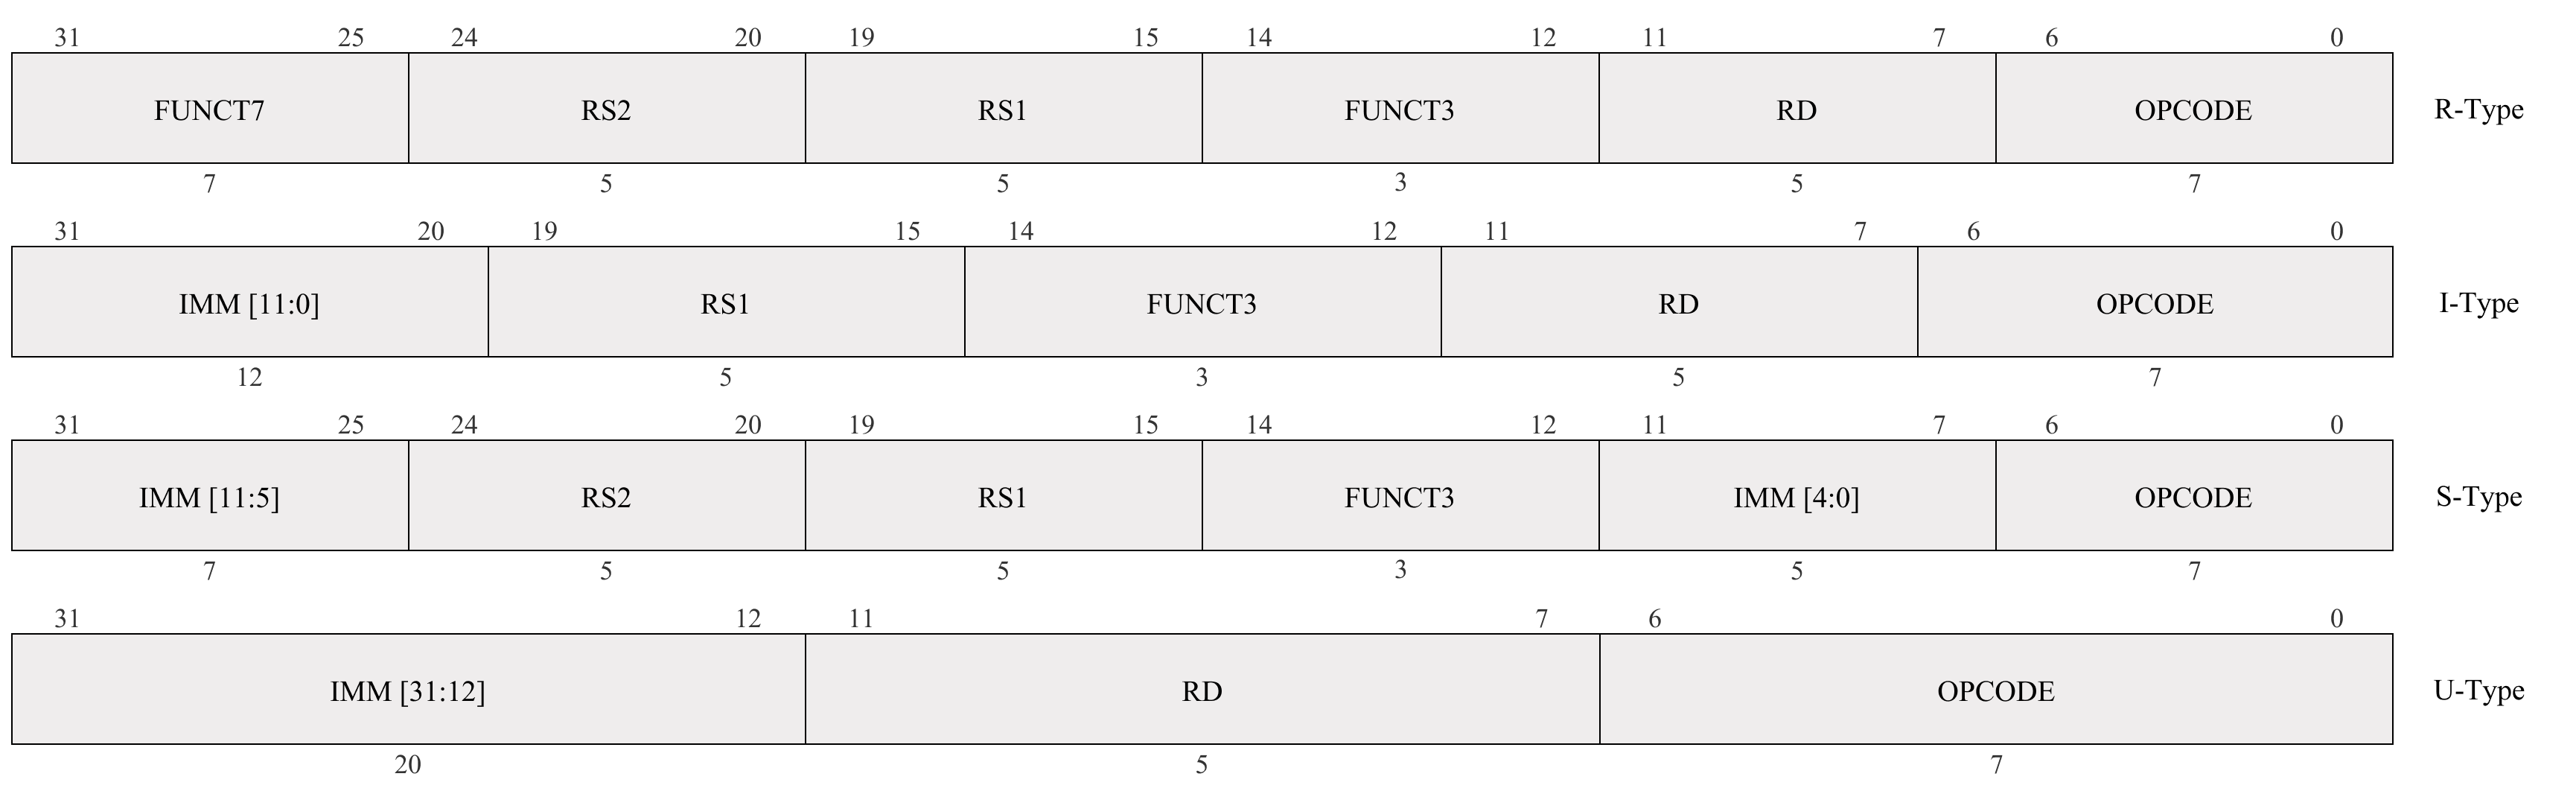
\includegraphics[width=.9\linewidth]{images/instrformats.png}}
  {\scriptsize }
  \caption{RISC-V Base Instruction Formats}
  \label{fig:instrformats}
\end{figure}

\begin{figure}[htbp]
  \centering
  \def\stackalignment{r}\stackunder{ 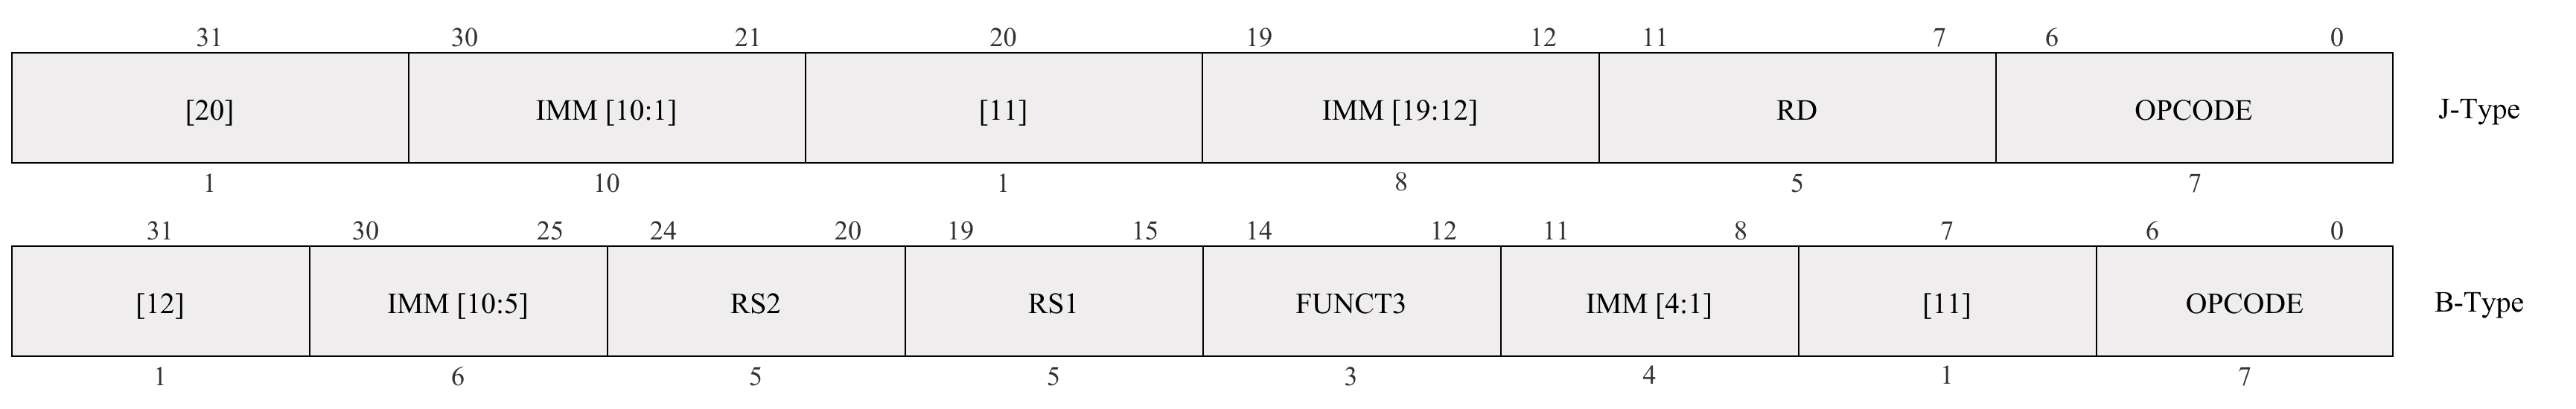
\includegraphics[width=.9\linewidth]{images/extrainstrformats.png} } %
  {\scriptsize }
  \caption{RISC-V Extra Instruction Formats}
  \label{fig:extrainstrformats}
\end{figure}

\section{RISC-V Exceptions, Traps and Interrupts}
\label{sec:riscv_eti}

In RISC-V, exceptions are unusual conditions tied to the execution of an instruction
within the hart, while interrupts are external asynchronous events that disrupt
normal execution. Both exceptions and interrupts lead to a trap, which transfers
control to a trap handler.

Traps in RISC-V can have four possible effects, each corresponding to how the trap
is managed:

\begin{itemize}
  \item Contained Trap: The trap is visible to software in the current
    environment and is handled within it. For example, a user-mode system call
    transfers control to a supervisor-mode handler.

  \item Requested Trap: A synchronous exception explicitly requests an action
    from the environment. The software may not resume execution on the hart afterward.

  \item Invisible Trap: The environment handles the trap transparently, so the running
    software is unaware of it. Examples include handling page faults or device
    interrupts, with execution continuing normally afterward.

  \item Fatal Trap: This indicates a critical failure, causing the environment to
    terminate execution, such as a virtual-memory protection failure.
\end{itemize}

As we will see later, traps are handled thanks to a trap vector table which is responsible
to manage the trap, decide the outcome, and resume the execution when needed.

\section{RISC-V Privilege Levels}
\label{sec:riscv_privileges}

RISC-V defines multiple privilege levels to manage access to system resources
and control execution modes. These privilege levels are designed to provide a secure
and efficient framework for managing different software components, such as
operating systems, hypervisors, and user applications.

As it's possible to see in Table \ref{tab:priv} RISC-v implements three
different privilege levels with the following characteristics:

\begin{itemize}
  \item Machine Mode (M-mode): Machine mode is the most privileged and
    fundamental level in the RISC-V architecture. It is the only required privilege
    level in all RISC-V implementations and provides complete access to hardware
    resources and system configurations. It is responsible for configuring the
    hardware, setting up system resources, and initializing other privilege
    levels. Furthermore, Trap Handling is performed by M-mode has;

  \item Supervisor Mode (S-mode): Supervisor mode is an optional privilege level
    designed for running operating systems or hypervisors. It offers more privileges
    than U-mode but less than M-mode. S-mode enables an operating system to
    manage resources and control hardware with enough authority while ensuring
    that user applications cannot access or alter critical system configurations;

  \item User Mode (U-mode): User mode is the least privileged level and is
    designed for running user-level applications. It restricts access to critical
    system resources, ensuring that any malicious or faulty application cannot
    compromise the overall system. U-mode’s restricted environment makes it ideal
    for running user applications securely, providing a balance between
    performance and protection.
\end{itemize}

\begin{table}
  \centering
  \begin{tabular}{|c|c|c|c|}
    \hline
    \textbf{Level} & \textbf{Encoding} & \textbf{Name}    & \textbf{Abbreviation} \\
    \hline
    0              & 00                & User/Application & U                     \\
    \hline
    1              & 01                & Supervisor       & S                     \\
    \hline
    2              & 10                & Reserved         &                       \\
    \hline
    3              & 11                & Machine          & M                     \\
    \hline
  \end{tabular}
  \caption{RISC-V privilege levels}
  \label{tab:priv}
\end{table}

\section{RISC-V General Purpose Registers}
\label{sec:riscv_reg}

The base RISC-V ISA provides $32$ general purpose registers all $32$ bits wide.
Table \ref{tab:registers} depicts all the described registers.

Except for \texttt{x0} which is hardwired to $0$ no other registers are assigned
to a specific role. However, the standard calling convention uses:
\begin{itemize}
  \item register x1: holds the return address for a call;

  \item register x5: serves as an alternate link register;

  \item register x2: as the stack pointer;

  \item \texttt{t}-registers: as temporary registers which are to be saved by the
    caller when needed;

  \item \texttt{a}-registers: as function arguments and return values;

  \item \texttt{s}-registers: as saved registers which are to be saved by the callee
    when needed.
\end{itemize}

\begin{table}
  \centering
  \begin{tabular}{|c|c|c|}
    \hline
    \textbf{Register} & \textbf{Alias} & \textbf{Calling Convention Description}    \\
    \hline
    x0                & zero           & Hard-wired zero                            \\
    \hline
    x1                & ra             & Return address                             \\
    \hline
    x2                & sp             & Stack pointer                              \\
    \hline
    x3                & gp             & Global pointer                             \\
    \hline
    x4                & tp             & Thread pointer                             \\
    \hline
    x5                & t0             & Temporary register/alternate link register \\
    \hline
    x6-x7             & t1-t2          & Temporary register                         \\
    \hline
    x8                & s0/fp          & Saved register/frame pointer               \\
    \hline
    x9                & s1             & Saved register                             \\
    \hline
    x10-x11           & a0-a1          & Function argument/return value             \\
    \hline
    x12-x17           & a2-a7          & Function argument                          \\
    \hline
    x18-x27           & s2-s11         & Saved register                             \\
    \hline
    x28-x32           & t3-t6          & Temporary register                         \\
    \hline
  \end{tabular}
  \caption{RISC-V general purpose registers}
  \label{tab:registers}
\end{table}

\section{RISC-V Control and Status Registers (CSRs)}
\label{sec:riscv_csrs}

RISC-V defines a separate address space of 4096 Control and Status Registers (CSRs)
which are particular registers used to control specific functions of the machine.
These special registers are mainly used by the Machine privilege thanks to the
following special instructions:
\begin{itemize}
  \item CSRRW (Atomic Read/Write CSR): atomically swaps values in the CSRs and
    integer registers. CSRRW reads the old value of the CSR and writes it to the
    destination register. The initial value in the source register is written to
    the CSR. If the destination register is x0, then the instruction will not
    read the CSR;

  \item CSRRS (Atomic Read and Set Bits in CSR): reads the value of the CSR and
    writes it to the destination register. The initial value in the source register
    is treated as a bit mask that specifies bit positions to be set in the CSR;

  \item CSRRC (Atomic Read and Clear Bits in CSR): reads the value of the CSR
    and writes it to the destination register. The initial value in the source register
    is treated as a bit mask that specifies bit positions to be cleared in the CSR.
\end{itemize}

Table \ref{tab:csrop} depicts whether a CSR is read or written by every
operation.
\begin{table}
  \centering
  \begin{tabular}{|c|c|c|c|c|}
    \hline
    \textbf{Instruction} & \textbf{Destination reg is x0} & \textbf{Source reg is x0} & \textbf{Reads CSR} & \textbf{Writes CSR} \\
    \hline
    CSRRW                & Yes                            & -                         & No                 & Yes                 \\
    \hline
    CSRRW                & No                             & -                         & Yes                & Yes                 \\
    \hline
    CSRRS/CSRRC          & -                              & Yes                       & Yes                & No                  \\
    \hline
    CSRRS/CSRRC          & -                              & No                        & Yes                & Yes                 \\
    \hline
  \end{tabular}
  \caption{CSR operation outcome}
  \label{tab:csrop}
\end{table}

Out of all the CSRs, only a few will be described since they will be necessary to
understand the functioning of this project.

\subsection{Machine Status Register (MSTATUS) CSR}
\label{subsec:mstatus}

The mstatus register keeps track of and controls the hart’s current operating
state. This register will be used to manage interrupts and privilege levels.
Figure \ref{fig:mstatus} depicts a representation of the mstatus CSR.

\begin{figure}[htbp]
  \centering
  \def\stackalignment{r}\stackunder{ 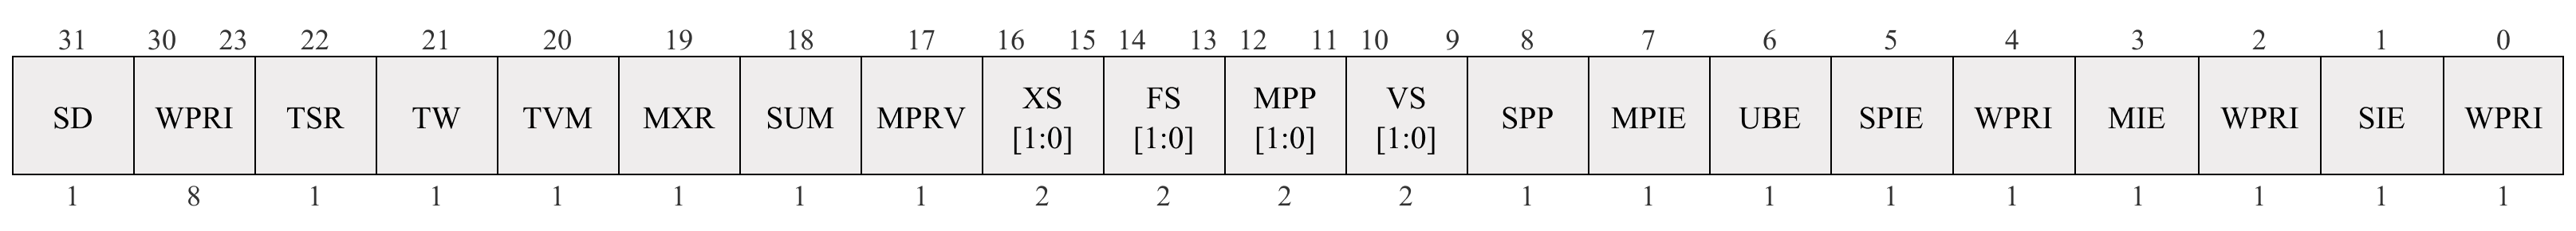
\includegraphics[width=.9\linewidth]{images/mstatus_csr.png} } %
  {\scriptsize }
  \caption{Machine status register}
  \label{fig:mstatus}
\end{figure}

\subsection{Machine Exception Program Counter (MEPC) CSR}
\label{subsec:mepc}

The mepc register is used, when a trap occurs, to store the address of the
instruction that was interrupted. Figure \ref{fig:mepc} depicts a representation
of the mepc CSR.

\begin{figure}[htbp]
  \centering
  \def\stackalignment{r}\stackunder{ 
\includegraphics[width=.9\linewidth]{images/mepc_csr.png} } %
  {\scriptsize }
  \caption{Machine Exception Program Counter}
  \label{fig:mepc}
\end{figure}

\subsection{Machine Cause Register (MCAUSE) CSR}
\label{subsec:mcause}

The mcause register is used, when a trap occurs, to store the code that indicates
the event that caused the trap. All the possible codes can be seen in Table
\ref{tab:causes}. Figure \ref{fig:mcause} depicts a representation of the mcause
CSR.

\begin{figure}[htbp]
  \centering
  \def\stackalignment{r}\stackunder{ 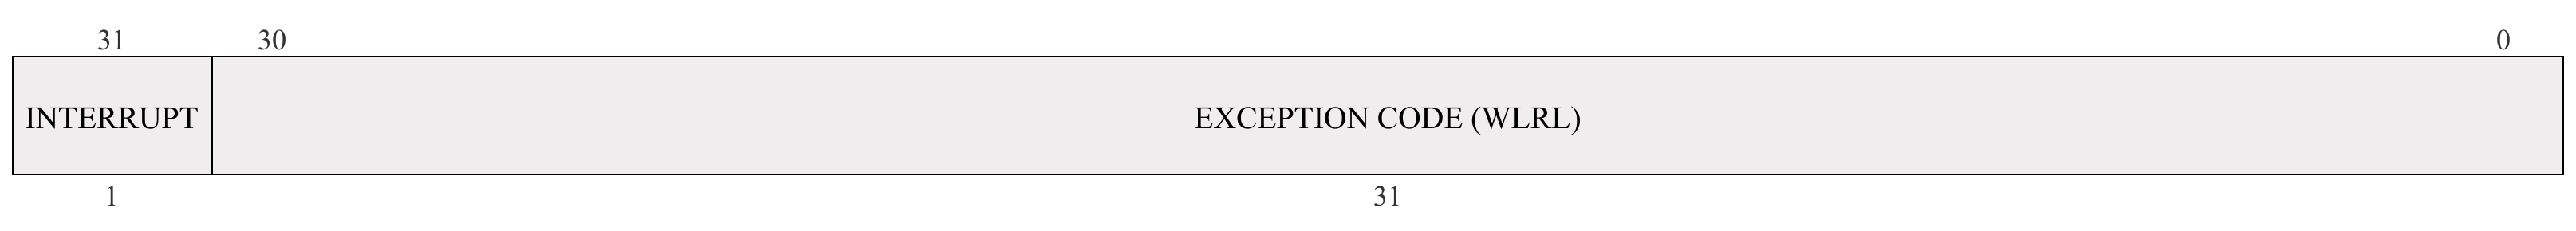
\includegraphics[width=.9\linewidth]{images/mcause_csr.png} } %
  {\scriptsize }
  \caption{Machine Cause Register}
  \label{fig:mcause}
\end{figure}

\begin{table}
  \centering
  \begin{tabular}{|c|c|c|}
    \hline
    \textbf{Interrupt} & \textbf{Code} & \textbf{Description}           \\
    \hline
    1                  & 0             & User software interrupt        \\
    \hline
    1                  & 1             & Supervisor software interrupt  \\
    \hline
    1                  & 2             & Reserved                       \\
    \hline
    1                  & 3             & Machine software interrupt     \\
    \hline
    1                  & 4             & User timer interrupt           \\
    \hline
    1                  & 5             & Supervisor timer interrupt     \\
    \hline
    1                  & 6             & Reserved                       \\
    \hline
    1                  & 7             & Machine timer interrupt        \\
    \hline
    1                  & 8             & User external interrupt        \\
    \hline
    1                  & 9             & Supervisor external interrupt  \\
    \hline
    1                  & 10            & Reserved                       \\
    \hline
    1                  & 11            & Machine external interrupt     \\
    \hline
    1                  & $\geq 12$     & Reserved                       \\
    \hline
    0                  & 0             & Instruction address misaligned \\
    \hline
    0                  & 1             & Instruction access fault       \\
    \hline
    0                  & 2             & Illegal instruction            \\
    \hline
    0                  & 3             & Breakpoint                     \\
    \hline
    0                  & 4             & Load address misaligned        \\
    \hline
    0                  & 5             & Load access fault              \\
    \hline
    0                  & 6             & Store/AMO address misaligned   \\
    \hline
    0                  & 7             & Store/AMO access fault         \\
    \hline
    0                  & 8             & Environment call from U-mode   \\
    \hline
    0                  & 9             & Environment call from S-mode   \\
    \hline
    0                  & 10            & Reserved                       \\
    \hline
    0                  & 11            & Environment call from M-mode   \\
    \hline
    0                  & 12            & Instruction page fault         \\
    \hline
    0                  & 13            & Load page fault                \\
    \hline
    0                  & 14            & Reserved                       \\
    \hline
    0                  & 15            & Store/AMO page fault           \\
    \hline
    0                  & 16-17         & Reserved                       \\
    \hline
    0                  & 18            & Software check                 \\
    \hline
    0                  & 19            & Hardware check                 \\
    \hline
    0                  & 20-23         & Reserved                       \\
    \hline
    0                  & 24-31         & Designated for custom use      \\
    \hline
    0                  & 32-47         & Reserved                       \\
    \hline
    0                  & 48-63         & Designated for custom use      \\
    \hline
    0                  & $\geq 64$     & Designated for custom use      \\
    \hline
  \end{tabular}
  \caption{Interrupts and Exception causes}
  \label{tab:causes}
\end{table}

\subsection{Machine Trap-Vector Base-Address Register (MTVEC) CSR}
\label{subsec:mtvec}

The mtvec register is used to store the address that holds the trap vector
configuration. Figure \ref{fig:mtvec} depicts a representation of the mtvec CSR.
The MODE field can be set according to Table \ref{tab:mode}. If we set the MODE to
Vectored, all asynchronous interrupts will set the program counter to the base
address encoded in mtvec plus $4$ times the cause of the interrupt (causes can be
seen in Table \ref{tab:causes}). With MODE set to Direct instead, all traps set
the program counter to the base address.

\begin{figure}[htbp]
  \centering
  \def\stackalignment{r}\stackunder{ 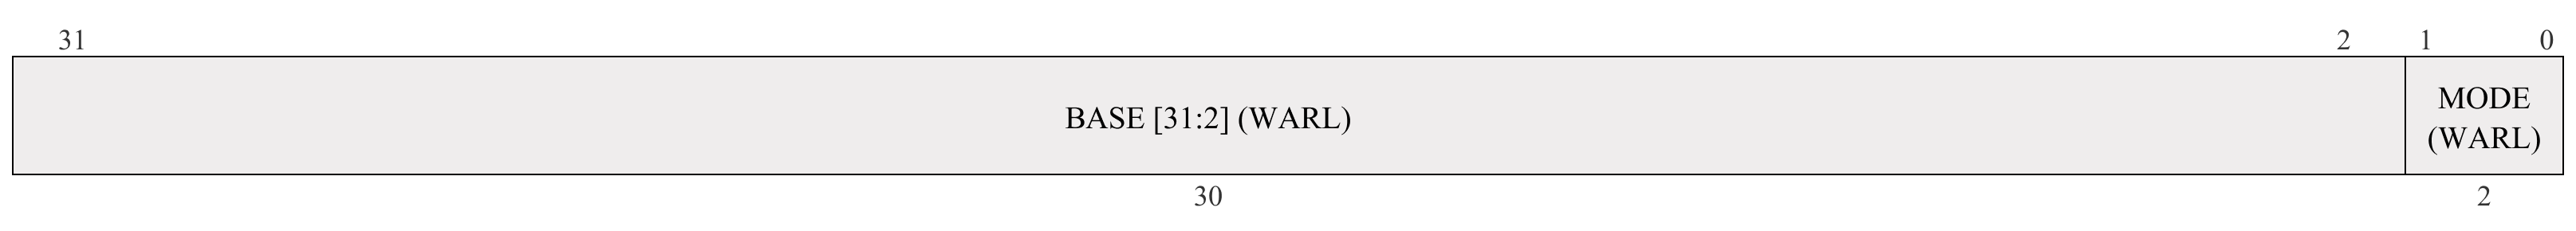
\includegraphics[width=.9\linewidth]{images/mtvec_csr.png} } %
  {\scriptsize }
  \caption{Machine Trap-Vector Base-Address Register}
  \label{fig:mtvec}
\end{figure}

\begin{table}
  \centering
  \begin{tabular}{|c|c|c|}
    \hline
    \textbf{Value} & \textbf{Name} & \textbf{Description}                             \\
    \hline
    $0$            & Direct        & All traps set pc to BASE                         \\
    \hline
    $1$            & Vectored      & Asynchronous interrupts set pc to $BASE+4*cause$ \\
    \hline
    $\geq 2$       & -             & Reserved                                         \\
    \hline
  \end{tabular}
  \caption{Encoding of MODE}
  \label{tab:mode}
\end{table}

\section{RISC-V Physical Memory Protection (PMP)}
\label{sec:riscv_pmp}

RISC-V provides an optional Physical Memory Protection (PMP) unit that allows to
configure access privileges (read, write, and execute) for each physical memory region.
The PMP ensures secure processing and helps to contain faults.

PMP checks are applied at all accesses in S or U mode. Optionally, PMP checks
may additionally apply to M-mode accesses, in which case the PMP registers themselves
are locked, so that even M-mode software cannot change them until the hart is
reset. Each PMP check results either in a violation which is trapped at the processor
or in a granted permission.

\subsection{PMP CSRs}

Each PMP entry is described by an 8-bit configuration register (pmpXcfg) and one
32-bit address register (pmpaddrX). Sixteen CSRs, pmpcfg0–pmpcfg15, hold the configurations
pmp0cfg–pmp63cfg for the 64 PMP entries (as shown in Figure \ref{fig:pmpcfgs}).
Each PMP address (pmpaddr0-pmpaddr63) encodes bits 33-2 of a 34-bit physical
address as shown in Figure \ref{fig:pmpaddr}.

Each PMP configuration register (Figure \ref{fig:pmpconf}) contains:
\begin{itemize}
  \item R-bit: when set allows read access;

  \item W-bit: when set allows write access;

  \item X-bit: when set allows instruction execution;

  \item A-bits: used to set address matching mode (better explained in subsection
    \ref{subsec:pmpaddressmatching});

  \item L-bit: when set the configuration is locked, meaning that it can't be modified
    without a system reset.
\end{itemize}

\begin{figure}[htbp]
  \centering
  \def\stackalignment{r}\stackunder{ 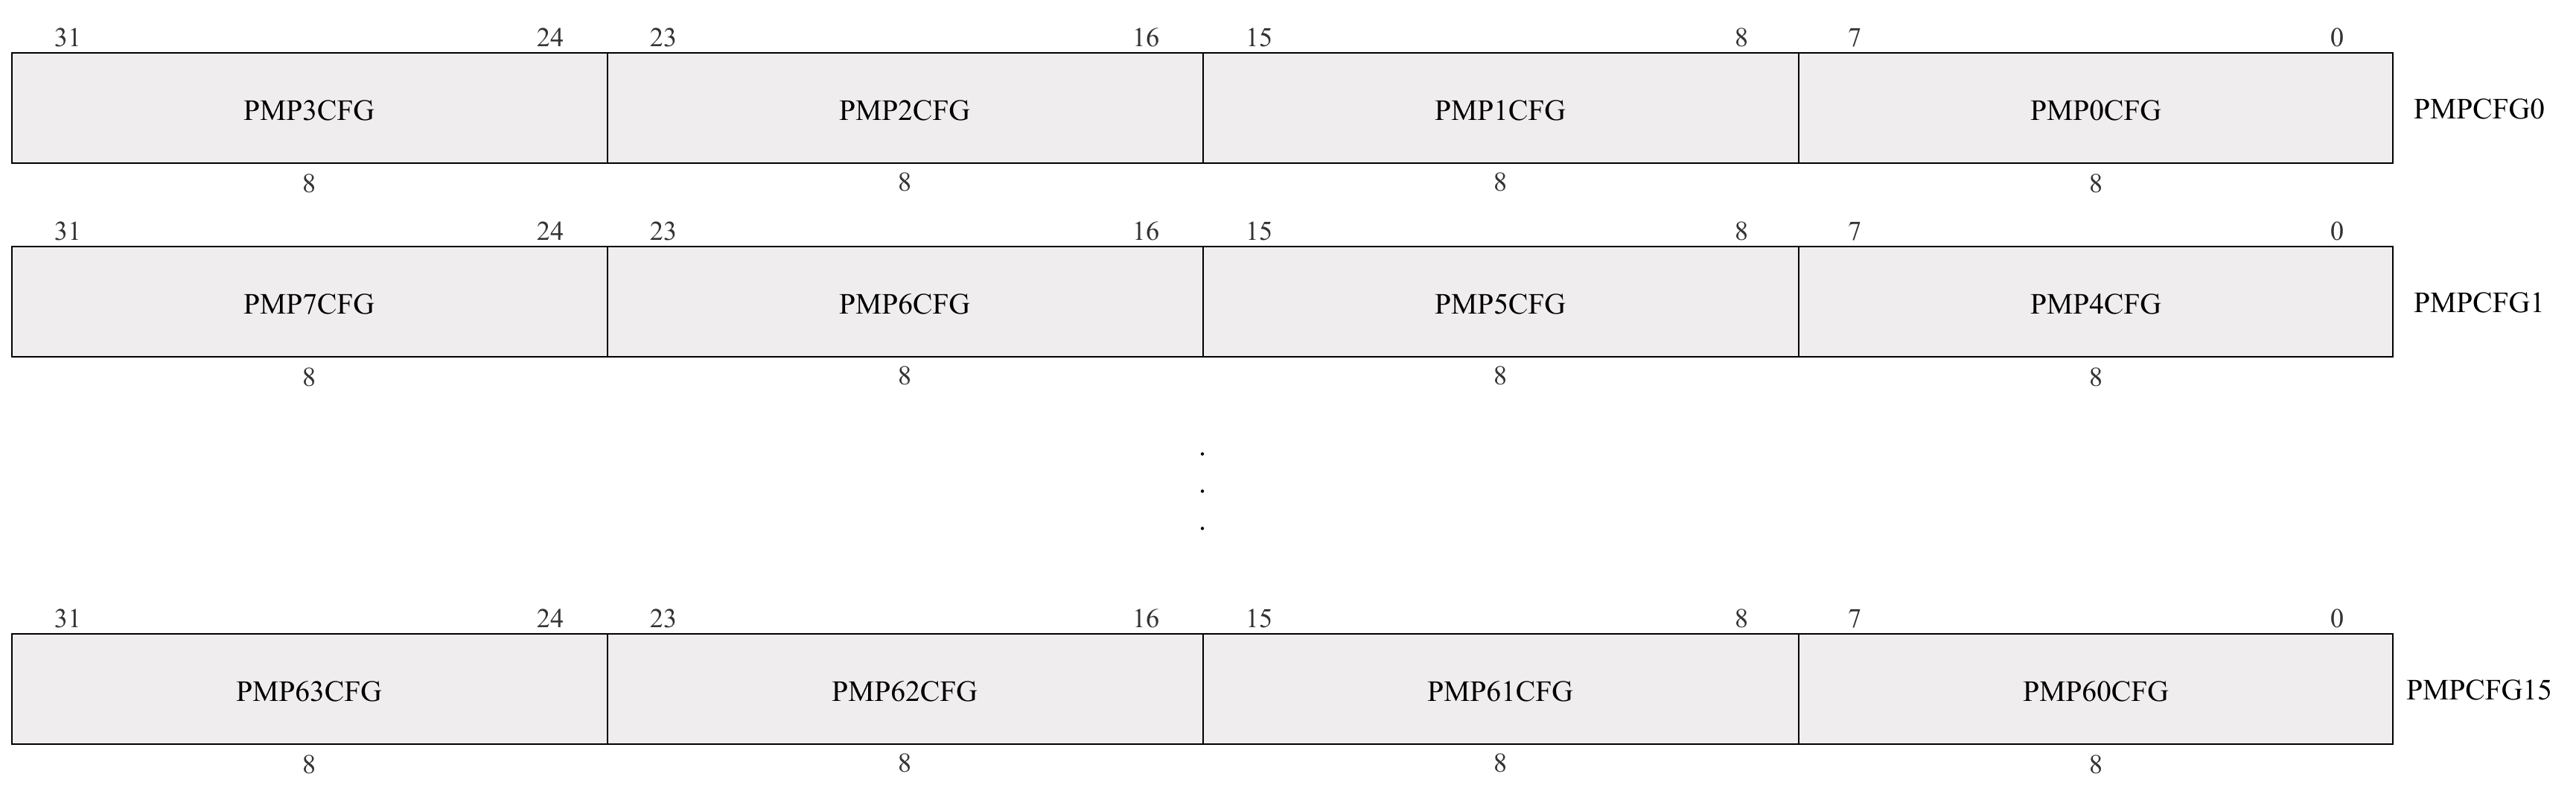
\includegraphics[width=.9\linewidth]{images/pmpcfgs_csr.png} } %
  {\scriptsize }
  \caption{PMP Configuration CSR}
  \label{fig:pmpcfgs}
\end{figure}

\begin{figure}[htbp]
  \centering
  \def\stackalignment{r}\stackunder{ 
\includegraphics[width=.9\linewidth]{images/pmpaddress_csr.png} } %
  {\scriptsize }
  \caption{PMP Configuration CSR}
  \label{fig:pmpaddr}
\end{figure}

\begin{figure}[htbp]
  \centering
  \def\stackalignment{r}\stackunder{ 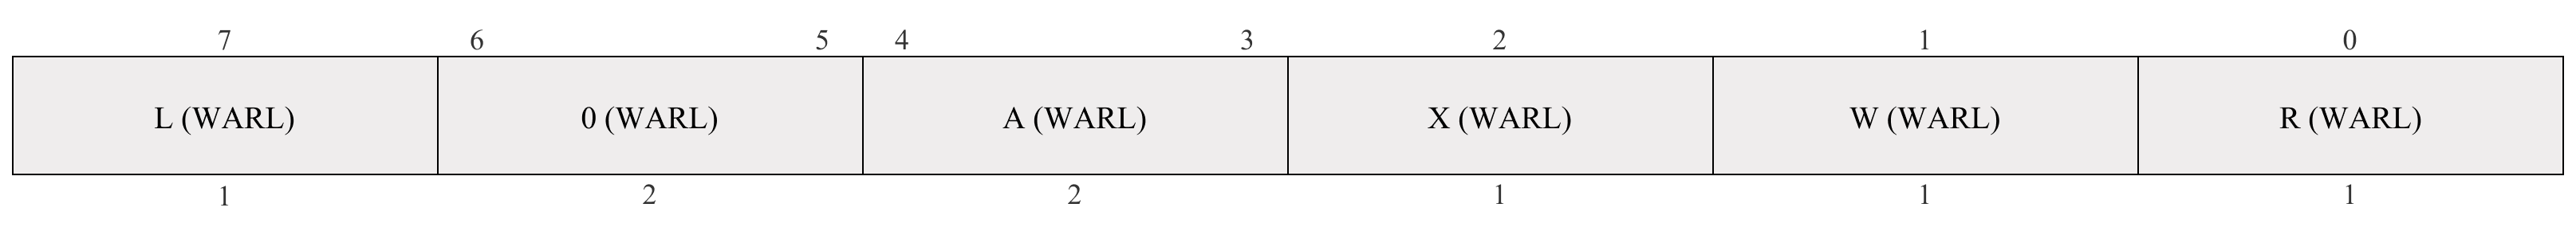
\includegraphics[width=.9\linewidth]{images/pmpconf_csr.png} } %
  {\scriptsize }
  \caption{PMP Configuration Register Format}
  \label{fig:pmpconf}
\end{figure}

\subsection{PMP Address Matching}
\label{subsec:pmpaddressmatching}

The A field in a PMP entry’s configuration register encodes the address-matching
mode of the associated PMP address register (encoding shown in Table \ref{tab:addressmatching}).

\begin{table}
  \centering
  \begin{tabular}{|c|c|c|}
    \hline
    \textbf{A} & \textbf{Name} & \textbf{Description}                  \\
    \hline
    00         & OFF           & Null region (disabled)                \\
    \hline
    01         & TOR           & Top of range                          \\
    \hline
    10         & NA4           & Naturally aligned four-byte region    \\
    \hline
    11         & NAPOT         & Naturally aligned power-of-two region \\
    \hline
  \end{tabular}
  \caption{Encoding of A in PMP Configuration Register}
  \label{tab:addressmatching}
\end{table}

When A=0, this PMP entry is disabled and matches no addresses. Two other address-matching
modes are supported:
\begin{itemize}
  \item Naturally aligned power-of-2 regions (NAPOT): NAPOT ranges make use of
    the low-order bits of the associated address register to encode the size of
    the range. This includes the special case of naturally aligned four-byte regions
    (NA4);

  \item Top boundary of an arbitrary range (TOR): If TOR is selected, the associated
    address register forms the top of the address range, and the preceding PMP
    address register forms the bottom of the address range. Note that, if the
    first PMP address is configured as TOR the lower boundary is considered to
    be 0x0.
\end{itemize}

\subsection{PMP Matching Logic}
\label{subsec:matchinglogic}

PMP entries are statically prioritized. The lowest-numbered PMP entry that matches
any byte of an access determines whether that access succeeds or fails. The
matching PMP entry must match all bytes of an access, or the access fails,
irrespective of the L, R, W, and X bits. For example, if a PMP entry is configured
to match the four-byte range 0xC–0xF, then an 8-byte access to the range 0x8–0xF
will fail, assuming that such PMP entry is the highest-priority entry that matches
those addresses.

If a PMP entry matches all bytes of an access, then the L, R, W, and X bits determine
whether the access succeeds or fails. If the L bit is clear and the privilege
mode of the access is M, the access succeeds. Otherwise, if the L bit is set or the
privilege mode of the access is S or U, then the access succeeds only if the R, W,
or X bit corresponding to the access type is set.

If no PMP entry matches an S-mode or U-mode access, but at least one PMP entry is
implemented, the access fails. Failed accesses generate a load, store, or instruction
access exception.